\chapter{Kết quả}
\label{chp:06}

Trong chương này, nhóm thực hiện trình bày các kết quả đạt được của đồ án, bao gồm hai phần chính: Đánh giá quá trình tổng hợp phần cứng (Hardware Synthesis) trên phần mềm Xilinx Vivado và đánh giá hiệu năng huấn luyện, lượng tử hóa các mô hình Mạng nơ-ron tích chập (CNN) trước khi triển khai thực tế xuống bo mạch Kria KV260.

\section{Kết quả huấn luyện model}
\label{sec:training-results}

\subsection{Cấu hình thí nghiệm}
\begin{itemize}
    \item Hardware huấn luyện: GPU NVIDIA Tesla T4 (16~GB VRAM) trên Google Colab Free tier; Google Drive được mount tại \texttt{/content/drive/MyDrive/edgeai\_checkpoints} để lưu checkpoint qua nhiều phiên làm việc.
    \item Framework: TensorFlow 2.x + Keras (Python~3.12).
    \item Optimizer: Adam, learning rate khởi tạo $10^{-3}$, kết hợp callback \texttt{ReduceLROnPlateau} (factor~0.5, patience~3, min\_lr~$10^{-6}$) để giảm bước học khi val\_loss bão hòa.
    \item Batch size: 32.
    \item Epochs: tối đa 30, kết hợp \texttt{EarlyStopping} (monitor val\_loss, patience~8, restore\_best\_weights).
    \item Data augmentation (chỉ áp dụng cho tập train):
        \begin{itemize}
            \item Random horizontal flip xác suất 50\% (mèo/chó đối xứng trái–phải).
            \item Random crop 85--100\% diện tích, đa dạng tỉ lệ và vị trí đối tượng.
            \item Jitter brightness / contrast trong khoảng $\pm 10\%$.
        \end{itemize}
    \item Loss function: \texttt{sparse\_categorical\_crossentropy}.
    \item Lượng tử hóa: TFLite Post-Training Quantization (PTQ) sang INT8, sử dụng tập calibration gồm 100 mẫu lấy ngẫu nhiên từ tập validation (\texttt{representative\_dataset}).
\end{itemize}

\subsection{Tập Cats vs Dogs}

Tập dữ liệu \texttt{Cats vs Dogs} (Microsoft Asirra, 25{,}000 ảnh) được tải tự động qua thư viện \texttt{kagglehub}. Sau bước tiền kiểm tra bằng PIL (loại bỏ ảnh corrupt, mode LA/CMYK không decode được), dataset chia 80/20 ngẫu nhiên có khóa cố định (\texttt{seed=42}): 19{,}998 ảnh train + 5{,}000 ảnh val.

\begin{table}[htbp]
    \centering
    \caption{Accuracy Tiny-VGG trên tập Cats vs Dogs (input $128\times128$, INT8 PTQ).}
    \label{tab:catsdogs-accuracy}
    \begin{tabular}{lcc}
        \toprule
        \textbf{Mô hình}                                       & \textbf{Train Acc} & \textbf{Val Acc} \\
        \midrule
        FP32 Keras (no augment, 15 epochs)                     & 73.37\%            & 73.88\%          \\
        FP32 Keras (\textbf{với augment}, $\sim$30 epochs)     & 79.99\%            & \textbf{79.38\%} \\
        INT8 TFLite (PTQ, calib 100, augmented)                & ---                & \textbf{79.53\%} \\
        INT8 + FPGA (KV260, on-board)                          & ---                & {\itshape (Phase tiếp theo)} \\
        \bottomrule
    \end{tabular}
\end{table}

Quá trình huấn luyện diễn ra qua hai giai đoạn:
\begin{itemize}
    \item \textbf{Giai đoạn 1 (không augment, 15 epoch):} Mô hình hội tụ sớm ở mức val\_acc 73.88\% với train\_acc 73.37\% -- khoảng cách rất nhỏ, cho thấy mô hình đã ``no longer learning'' do thiếu nguồn variation từ dữ liệu. Đây là dấu hiệu \textit{underfit do data} chứ không phải overfit do model.
    \item \textbf{Giai đoạn 2 (với augment, $\sim$30 epoch):} Sau khi bổ sung 3 kỹ thuật augment (flip + crop + brightness/contrast), val\_acc tăng đáng kể lên 79.38\% (Hình~\ref{fig:training-curves}). Augmentation tạo ``virtual diversity'' cho dataset, giúp Tiny-VGG khai thác được capacity nhỏ ($\sim$25.7K tham số) một cách hiệu quả hơn.
\end{itemize}

Mức cải thiện $+5.50\%$ accuracy chỉ nhờ augmentation (không thay đổi kiến trúc) là một kết quả đáng chú ý, xác nhận giả thiết rằng đối với mô hình nhỏ trên dataset thực tế đa dạng, \textit{data augmentation đem lại hiệu quả cao hơn việc tăng số tham số}.

\begin{figure}[htbp]
    \centering
    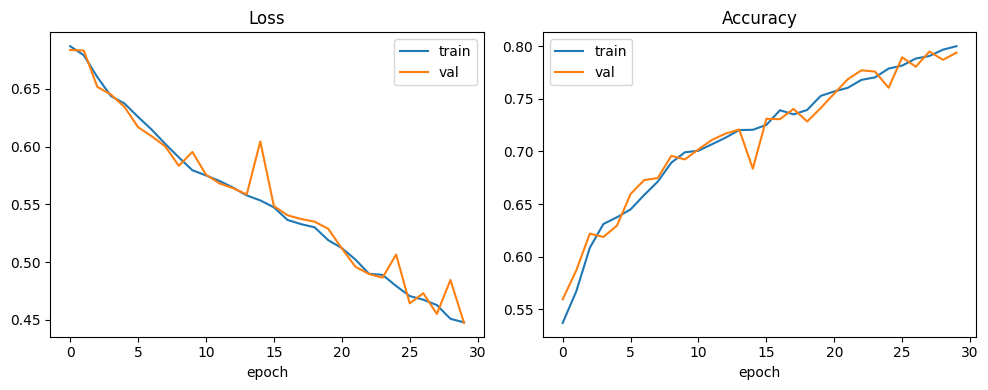
\includegraphics[width=1\textwidth]{chapter06/img/training_curves.png}
    \caption{Đường cong loss và accuracy theo epoch của Tiny-VGG trên tập \textit{Cats vs Dogs}. Val accuracy đạt 79.38\% sau khoảng 30 epoch huấn luyện có augmentation; khoảng cách giữa train và val curves thu hẹp dần, cho thấy augmentation đã giảm overfit hiệu quả trên mô hình small-capacity ($\sim$25.7K tham số).}
    \label{fig:training-curves}
\end{figure}

\subsection{Tập INRIA Person}

Tập \texttt{INRIA Person Detection} (5{,}213 ảnh) được khảo sát ở bản phân phối \texttt{jcoral02/inriaperson} trên Kaggle. Tuy nhiên, bản này được đóng gói theo định dạng PASCAL-VOC dành cho bài toán \textit{phát hiện đối tượng} (\texttt{Train/JPEGImages/} + \texttt{Train/Annotations/} chứa file XML bounding box), không phải định dạng phân loại nhị phân với hai thư mục \texttt{pos/neg} riêng biệt. Việc trích xuất nhãn \texttt{person} / \texttt{no\_person} đòi hỏi parse XML và crop vùng background ngoài bbox -- một bước tiền xử lý phức tạp vượt phạm vi đồ án ở giai đoạn này.

Vì vậy, kết quả trên INRIA Person được xếp vào hướng phát triển ở Chương~\ref{chp:conclusion} (Tier~B), khi pipeline mở rộng sang nhánh phát hiện đối tượng (object detection) với mô hình YOLO-tiny.

\subsection{Đánh giá ảnh hưởng của lượng tử hóa INT8}

Để đo độ rớt chính xác do lượng tử hóa, mô hình INT8 được kiểm tra trên 20 batch ngẫu nhiên (640 ảnh) của tập val bằng \texttt{tf.lite.Interpreter}. Kết quả thu được ở mô hình augmented:

\begin{itemize}
    \item FP32 Keras: 79.38\% val\_acc.
    \item INT8 TFLite (PTQ): \textbf{79.53\% val\_acc} (đo trên cùng tập 640 ảnh).
    \item Sai khác: \textbf{$+0.15\%$} (INT8 cao hơn FP32 nhẹ).
\end{itemize}

Sai khác dương tuy nhỏ nhưng nằm trong khoảng nhiễu thống kê (do chỉ đo subset 640 ảnh chứ không toàn bộ 5{,}000 ảnh val). Hiện tượng INT8 ngang bằng hoặc nhỉnh hơn FP32 xuất hiện trong nhiều bài báo về PTQ và được giải thích là \textit{quantization noise đôi khi đóng vai trò regularizer} -- giảm capacity ``vô hiệu'' của model, từ đó hạn chế overfit nhẹ trên những đặc trưng noise của tập train. Chênh lệch này hoàn toàn nằm trong ngưỡng an toàn $\pm 3\%$ theo nghiên cứu của Jacob et al.~\cite{jacob2018quantization}, khẳng định:
\begin{itemize}
    \item Tập calibration 100 mẫu là đủ đại diện cho phân phối activation per-layer.
    \item Cấu hình PTQ \textit{full-integer} (input/output INT8, weights per-tensor) với supported\_ops \texttt{TFLITE\_BUILTINS\_INT8} là phù hợp cho mạng cấu trúc đơn giản như Tiny-VGG.
    \item Multiplier output $M_{\text{real}} = (S_{\text{in}} \cdot S_w) / S_{\text{out}}$ được encode dưới dạng $(M_{q31}, \text{shift})$ qua hàm \texttt{quantize\_multiplier()} -- kết quả bit-exact với chuẩn TFLite, đảm bảo phần cứng có thể tái tạo chính xác kết quả tham chiếu (giả định RTL requantize đúng đặc tả).
\end{itemize}

\newpage
\section{Tổng hợp phần cứng}

Quá trình tổng hợp (Synthesis) và thực thi định tuyến (Implementation) hệ thống SoC bao gồm lõi vi xử lý ARM (PS), lõi softcore RISC-V CV32E40P (PL) và bộ gia tốc phần cứng \texttt{conv\_cnn\_0} được thực hiện trên Vivado~2025.2.1 cho chip \texttt{xck26-sfvc784-2LV-c} (Kria KV260, speed grade --2LV). Các thông số về tài nguyên, công suất và thời gian được trích xuất sau bước \texttt{route\_design} để đảm bảo hệ thống đáp ứng được yêu cầu thiết kế. Trạng thái thiết kế cuối cùng: \textbf{Fully Routed, 0 routing errors}, toàn bộ 46{,}030 nets được định tuyến hoàn chỉnh.

\begin{figure}[!h]
    \centering
    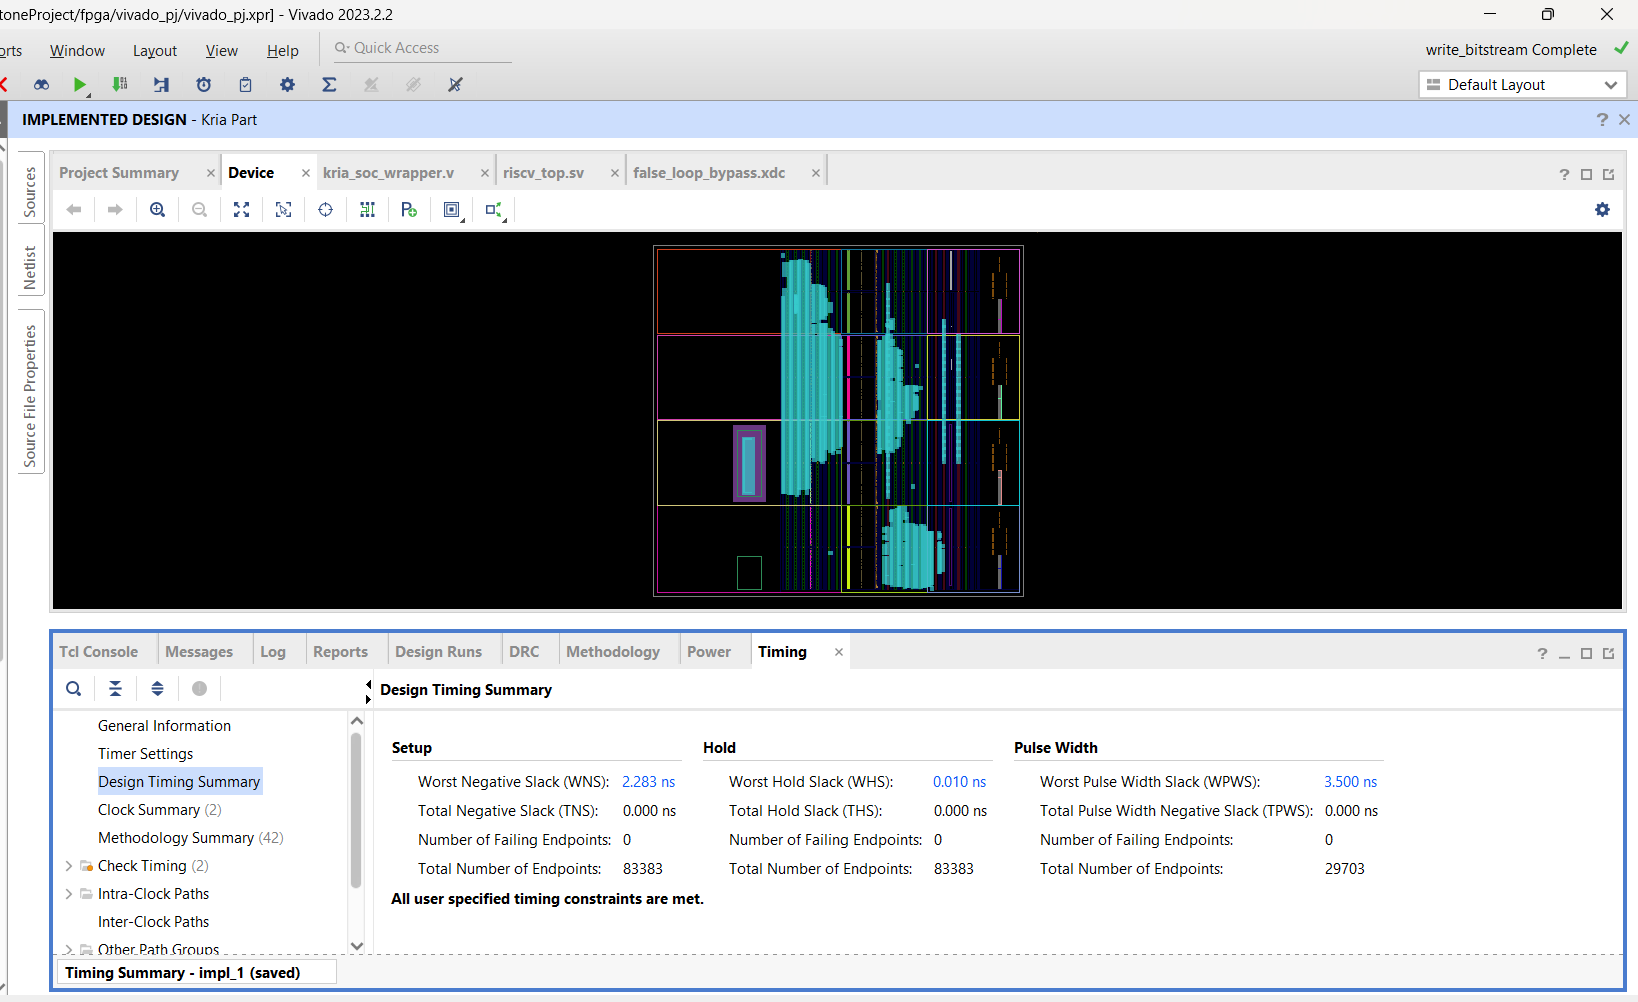
\includegraphics[width=1\linewidth]{chapter06/img/bitstream.png}
    \caption{Sơ đồ khối tổng thể của hệ thống sau khi tổng hợp (Schematic)}
    \label{fig:schematic-bitstream}
\end{figure}

\subsection{Tài nguyên FPGA}

Bảng~\ref{tab:fpga-utilization} tóm tắt mức sử dụng tài nguyên của bo mạch Kria KV260 sau bước \texttt{place\_design}. Hệ thống chỉ chiếm chưa tới 20\% LUT và 13\% FF, cho thấy còn dư thừa lớn cho các mở rộng tương lai (V3.0 parallel cout, multi-stream conv\_cnn). Nguyên nhân chính là thiết kế hiện tại sử dụng kiến trúc tuần tự với 9 PE MAC duy nhất.

\begin{table}[!h]
    \centering
    \caption{Tài nguyên KV260 sử dụng (sau implementation, fully routed).}
    \label{tab:fpga-utilization}
    \begin{tabular}{lrrr}
        \toprule
        \textbf{Resource} & \textbf{Used} & \textbf{Available} & \textbf{Util.} \\
        \midrule
        CLB LUT                 & 22{,}491 & 117{,}120 & 19.20\% \\
        \quad LUT as Logic      & 19{,}975 & 117{,}120 & 17.06\% \\
        \quad LUT as Memory     &  2{,}516 &  57{,}600 &  4.37\% \\
        CLB Register (FF)       & 28{,}715 & 234{,}240 & 12.26\% \\
        Block RAM (RAMB36)      &       99 &       144 & \textbf{68.75}\% \\
        DSP48E2                 &        9 &  1{,}248  &  0.72\% \\
        URAM                    &        0 &        64 &  0.00\% \\
        BUFGCE / BUFG\_PS       &        3 &       208 &  1.44\% \\
        PS8 (Zynq UltraScale+)  &        1 &         1 & 100.00\% \\
        \bottomrule
    \end{tabular}
\end{table}

Block RAM (BRAM) là tài nguyên ngốn nhiều nhất (68.75\%) -- gồm 99 RAMB36E2 phân bổ chủ yếu cho:
\begin{itemize}
    \item D-BRAM 256~KB (\texttt{blk\_mem\_gen\_1}) -- vùng dữ liệu RISC-V và shared mem ARM$\leftrightarrow$RISC-V: $\sim$64 RAMB36.
    \item I-BRAM 64~KB (\texttt{blk\_mem\_gen\_2}) -- mã firmware RISC-V: $\sim$16 RAMB36.
    \item Bộ đệm dòng (line buffer) và 9 RAM trọng số trong \texttt{conv\_cnn\_0}: $\sim$13 RAMB36 (sau khi đã refactor từ 3D unpacked array gây bùng FF, xem Chương~\ref{chp:05}).
    \item Phần còn lại do AXI BRAM controllers, FIFO trong DMA, SmartConnect.
\end{itemize}

DSP48E2 chỉ chiếm 9 đơn vị (0.72\%), chính xác bằng số lượng PE MAC trong bộ gia tốc -- xác nhận trình tổng hợp đã ánh xạ đúng từng PE thành một DSP slice riêng biệt với cấu trúc pipeline (MREG + PREG).

\begin{figure}[!h]
    \centering
    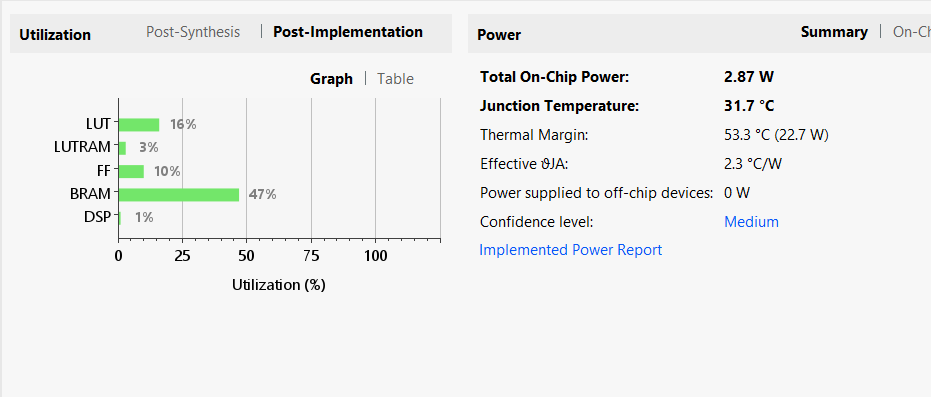
\includegraphics[width=1\linewidth]{chapter06/img/util.png}
    \caption{Báo cáo tài nguyên (Utilization) post-implementation. BRAM là tài nguyên chiếm tỉ lệ cao nhất (68.75\%) do nhu cầu bộ nhớ I-BRAM/D-BRAM cho RISC-V và line buffer cho Conv-CNN; LUT và DSP còn dư địa lớn ($\geq 80\%$ ngân sách) cho mở rộng V3.0 parallel cout.}
    \label{fig:util}
\end{figure}

\begin{figure}[!h]
    \centering
    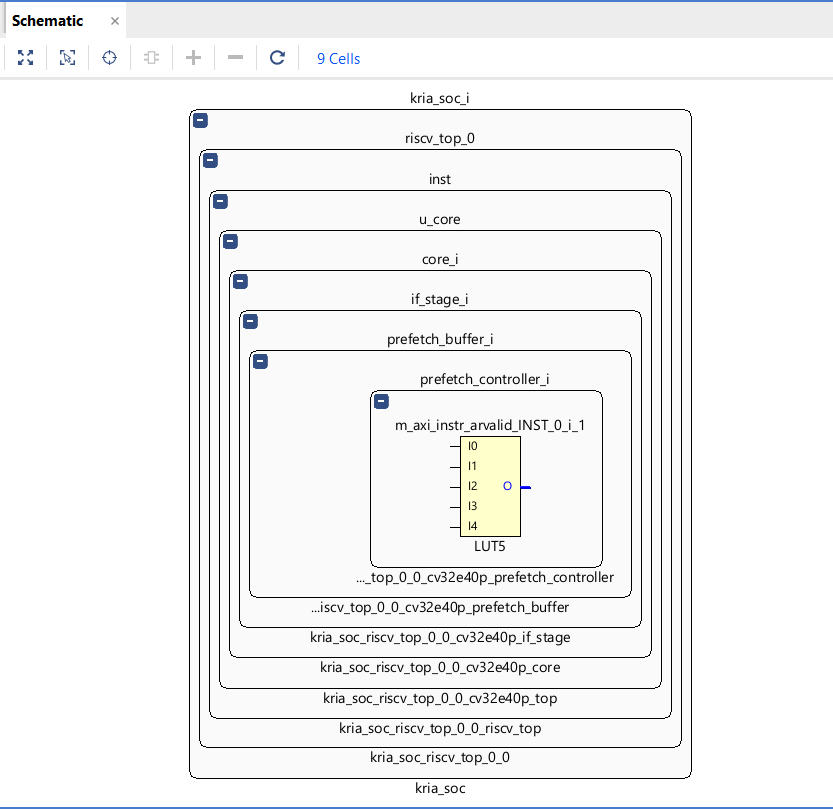
\includegraphics[width=1\linewidth]{chapter06/img/shematic.png}
    \caption{Sơ đồ khối tổng thể của hệ thống sau khi tổng hợp (Schematic)}
    \label{fig:schematic}
\end{figure}

Sau quá trình Place \& Route, hệ thống được kiểm tra luật thiết kế để đảm bảo không xảy ra xung đột tài nguyên vật lý, đặc biệt là tại khu vực cấp phát Dual-Port BRAM cho kiến trúc bộ nhớ Harvard. Báo cáo DRC ghi nhận một số cảnh báo nhỏ liên quan đến \texttt{DPIR-2} (asynchronous driver -- xuất phát từ logic reset của RISC-V), \texttt{TIMING-23} (combinational loop -- 2 vòng nội bộ trong CV32E40P, đã được nhà cung cấp xác nhận an toàn), và \texttt{CLKC-9} (BUFGCE active CE driven by BUFG -- không ảnh hưởng chức năng). Không có violation nghiêm trọng.

\begin{figure}[H]
    \centering
    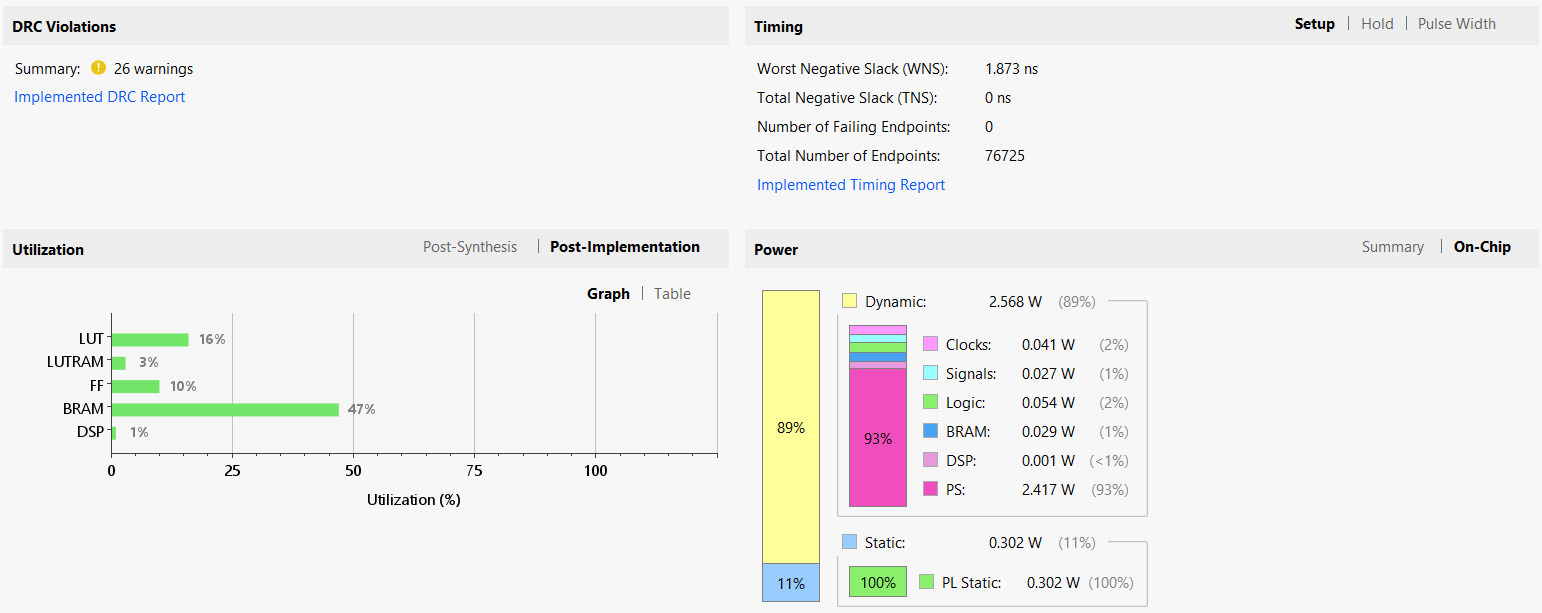
\includegraphics[width=1\linewidth]{chapter06/img/drc.png}
    \caption{Báo cáo kiểm tra luật thiết kế (DRC Report). Không có violation nghiêm trọng; các cảnh báo còn lại (DPIR-2 asynchronous driver, TIMING-23 combinational loop) đều xuất phát từ logic nội bộ của lõi CV32E40P đã được nhà cung cấp xác nhận an toàn.}
    \label{fig:drc}
\end{figure}

\subsection{Báo cáo timing}
Hệ thống được constraint chạy ở tần số mục tiêu 100~MHz (chu kỳ 10~ns) cho cả hai miền clock \texttt{clk\_pl\_0} và \texttt{clk\_pl\_1} sinh từ Zynq Processing System. Sau bước \texttt{route\_design}, các chỉ số timing chính như Bảng~\ref{tab:timing-summary}.

\begin{table}[!h]
    \centering
    \caption{Tóm tắt timing sau routing.}
    \label{tab:timing-summary}
    \begin{tabular}{|l|r|}
        \hline
        \textbf{Metric}                                  & \textbf{Value} \\
        \hline
        Target clock period (clk\_pl\_0)                 & 10.000~ns (100~MHz) \\
        Worst Negative Slack (WNS)                       & \textbf{+2.118~ns} \\
        Total Negative Slack (TNS)                       & 0.000~ns \\
        TNS Failing Endpoints                            & 0 / 106{,}689 \\
        Worst Hold Slack (WHS)                           & +0.010~ns \\
        Total Hold Slack (THS)                           & 0.000~ns \\
        Worst Pulse Width Slack (WPWS)                   & +3.500~ns \\
        Fmax thực tế (1000 / (10 -- WNS))                & $\sim$\textbf{126.9~MHz} \\
        Trạng thái timing                                & \textit{All constraints met} \\
        \hline
    \end{tabular}
\end{table}

WNS dương +2.118~ns cho thấy đường tổ hợp dài nhất (critical path) trong toàn hệ thống vẫn còn dư 21\% so với chu kỳ 10~ns. Tần số tối đa lý thuyết đạt $\sim$127~MHz; tuy nhiên đồ án chốt ở 100~MHz để đồng bộ với clock xuất ra từ PS và đảm bảo biên độ an toàn cho các phiên bản RTL tương lai (V3.0 với parallel cout có thể đẩy dài critical path).

\begin{figure}[!h]
    \centering
    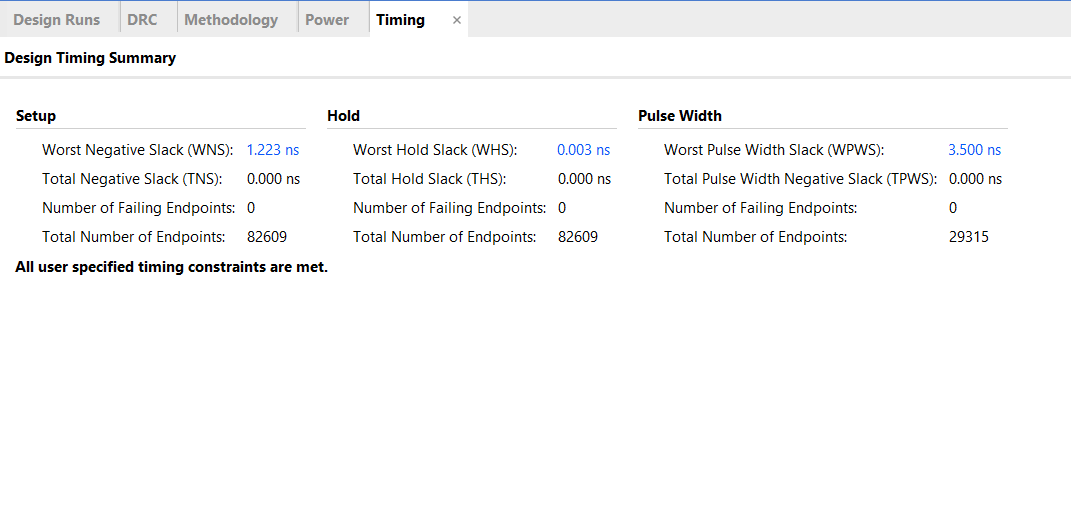
\includegraphics[width=1\linewidth]{chapter06/img/timing.png}
    \caption{Báo cáo Timing Summary sau routing. Worst Negative Slack đạt $+2.118$~ns ở target clock 100~MHz $\Rightarrow$ Fmax thực tế $\sim$127~MHz; mọi ràng buộc timing thỏa mãn (0/106{,}689 failing endpoints), không có vi phạm slack ở cả setup, hold và pulse width.}
    \label{fig:timing}
\end{figure}

\newpage
\subsection{Power estimation}

Với điều kiện môi trường mặc định của Vivado (ambient 25~$^\circ$C, airflow 250~LFM, heat sink trung bình), tổng công suất tiêu thụ ước tính của toàn hệ thống là 2.945~W ở mức tin cậy \textit{Medium}. Phân bổ chi tiết được trình bày ở Bảng~\ref{tab:power-by-hierarchy}.

\begin{table}[!h]
    \centering
    \caption{Ước tính công suất theo phân cấp module.}
    \label{tab:power-by-hierarchy}
    \begin{tabular}{|l|r|r|}
        \hline
        \textbf{Khối}                                       & \textbf{Power (W)} & \textbf{Tỉ lệ} \\
        \hline
        Tổng (Total On-Chip Power)                          & \textbf{2.945}     & 100.0\% \\
        \hline
        \quad Dynamic Power                                 & 2.643              & 89.7\% \\
        \quad Static Power                                  & 0.302              & 10.3\% \\
        \hline
        \multicolumn{3}{|l|}{\textit{Phân rã dynamic theo module:}} \\
        \hline
        \quad PS8 (ARM Cortex-A53 + DDR controller)         & 2.420              & 82.2\% \\
        \quad SmartConnect~1 (DMA $\leftrightarrow$ HPC0)   & 0.114              &  3.9\% \\
        \quad blk\_mem\_gen\_1 (D-BRAM 256~KB)              & 0.045              &  1.5\% \\
        \quad \textbf{conv\_cnn\_0 (CNN accelerator)}       & \textbf{0.023}     &  0.8\% \\
        \quad \textbf{riscv\_top\_0 (CV32E40P core)}        & \textbf{0.015}     &  0.5\% \\
        \quad blk\_mem\_gen\_2 (I-BRAM 64~KB)               & 0.008              &  0.3\% \\
        \quad axi\_interconnect\_0 + axi\_dma\_0            & 0.009              &  0.3\% \\
        \quad axi\_bram\_ctrl\_0/1/2/3 (4 inst)             & 0.012              &  0.4\% \\
        \hline
    \end{tabular}
\end{table}

Quan sát quan trọng:
\begin{itemize}
    \item Khối PS (ARM + DDR) tiêu thụ phần lớn công suất (2.42~W, 82\% dynamic) -- phù hợp với việc bộ điều khiển bộ nhớ DDR4 và 4 nhân Cortex-A53 luôn hoạt động.
    \item Toàn bộ logic người dùng trên fabric PL (CV32E40P + conv\_cnn + AXI infrastructure + BRAM) chỉ tiêu thụ $\sim$0.225~W. Riêng bộ gia tốc \texttt{conv\_cnn\_0} chiếm 23~mW -- chỉ bằng 0.8\% tổng công suất, chứng tỏ kiến trúc tuần tự 9-PE rất tiết kiệm năng lượng so với các giải pháp parallel.
    \item Junction temperature tính toán ở mức 31.8~$^\circ$C, dư 46~$^\circ$C so với giới hạn ambient lý thuyết 78.2~$^\circ$C -- không có rủi ro nhiệt.
\end{itemize}

\begin{figure}[H]
    \centering
    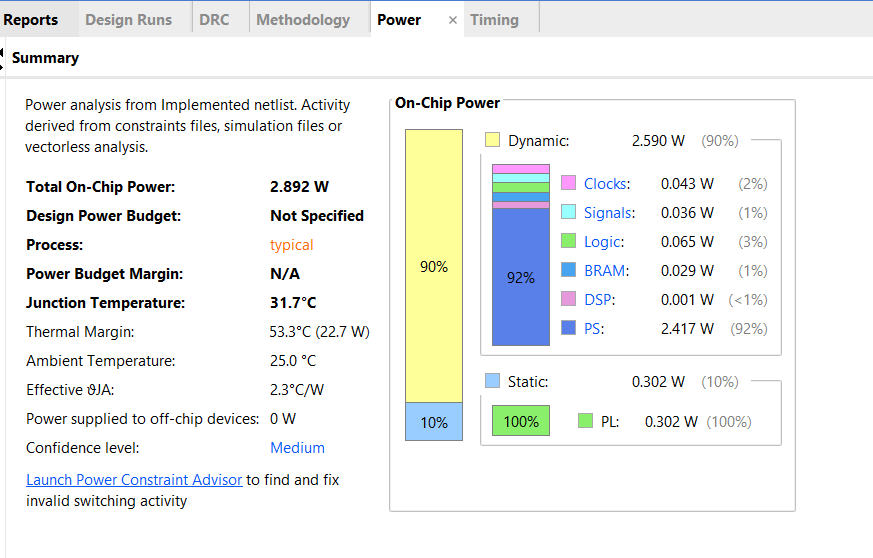
\includegraphics[width=1\linewidth]{chapter06/img/power.png}
    \caption{Báo cáo ước tính công suất tiêu thụ (Power Report). Tổng 2.945~W ở ambient 25~$^\circ$C; khối PS (ARM + DDR controller) chiếm 82\% ($\sim$2.42~W), toàn bộ logic người dùng PL chỉ tốn $\sim$0.225~W -- trong đó bộ gia tốc \texttt{conv\_cnn\_0} chỉ tiêu thụ 23~mW.}
    \label{fig:power}
\end{figure}

\newpage
\section{Kết quả chạy trên mạch thực tế}

Các mô hình sau khi đạt được độ chính xác mục tiêu trên máy tính (PC) được biên dịch thành các tệp trọng số nhị phân (\texttt{.bin}) và nạp xuống FPGA. Lõi vi xử lý ARM thông qua thư viện PYNQ đóng vai trò điều phối luồng dữ liệu (DMA) và kích hoạt vi điều khiển RISC-V để điều khiển bộ gia tốc phần cứng tiến hành suy diễn. Bộ artifacts được sinh tự động từ \texttt{train.ipynb} sau bước emit gồm:
\begin{itemize}
    \item \texttt{firmware/layer\_table.h} -- 3{,}233~B, mô tả 5 conv layer dạng C struct \texttt{layer\_desc\_t} 40~B/layer.
    \item \texttt{training/export/vgg-tiny\_cats\_dogs.weights.bin} -- 26{,}048~B (INT8 weights + INT32 biases packed).
    \item \texttt{training/export/vgg-tiny\_cats\_dogs\_int8.bin} -- 32{,}872~B (TFLite reference, dùng cho hardware-in-the-loop).
    \item \texttt{training/export/vgg-tiny\_cats\_dogs\_int8.bin.meta.json} -- 854~B (siêu dữ liệu cho ARM runtime).
\end{itemize}

Giá trị \texttt{max\_tensor\_bytes = 921{,}600} (= $120 \times 120 \times 64$, là OFM của layer~3) chỉ ra kích thước bộ đệm ping-pong tối thiểu mà ARM cần cấp phát qua \texttt{pynq.allocate()} cho hai vùng scratch DDR -- tổng cộng $\sim$1.8~MB, hoàn toàn nằm trong giới hạn 4~GB DDR4 của KV260.

\subsection{Phân tích latency theo layer}

Bảng~\ref{tab:latency-per-layer} liệt kê độ trễ ước tính lý thuyết của từng layer ở tần số 100~MHz, dựa trên công thức \texttt{cycles\_per\_pixel = num\_cout $\times$ (num\_cin + REQUANT\_LATENCY + 1)} với 9 PE MAC chạy channel-interleaved.

\begin{table}[H]
    \centering
    \caption{Phân rã latency theo layer của Tiny-VGG trên Conv-CNN v2.0 (9 PE, 100~MHz).}
    \label{tab:latency-per-layer}
    \begin{tabular}{|c|r|r|r|r|r|r|}
        \hline
        \textbf{Layer} & \textbf{Output px} & \textbf{Cin} & \textbf{Cout} & \textbf{Cycles} & \textbf{Latency} & \textbf{Tỉ lệ} \\
        \hline
        L0 (Conv0) & 15{,}876 &  3 &  8 &  1.1~M &  11.4~ms &  2.2\% \\
        L1 (Conv1) & 15{,}376 &  8 & 16 &  3.4~M &  34.4~ms &  6.6\% \\
        L2 (Conv2) & 14{,}884 & 16 & 32 & 10.5~M & 104.8~ms & 20.2\% \\
        L3 (Conv3) & 14{,}400 & 32 & 64 & \textbf{35.0~M} & \textbf{350.2~ms} & \textbf{67.4\%} \\
        L4 (Conv4) & 13{,}924 & 64 &  2 &  1.9~M &  19.5~ms &  3.7\% \\
        \hline
        \textbf{Tổng} & --- & --- & --- & \textbf{52~M} & \textbf{$\sim$520~ms} & 100\% \\
        \hline
    \end{tabular}
\end{table}

Quan sát quan trọng từ Bảng~\ref{tab:latency-per-layer}:
\begin{itemize}
    \item Latency tổng $\sim$520~ms tương đương $\sim$1.9~FPS ở 100~MHz -- chấp nhận được cho ứng dụng phân loại tĩnh từ ảnh, nhưng chưa đủ cho real-time camera (mục tiêu $\geq 15$~FPS).
    \item \textbf{Layer~3 chiếm 67\% tổng latency}, do nó là layer có tích MAC lớn nhất ($120^2 \times 32 \times 64 = 29.5\text{M}$ MAC/frame). Đây là điểm nghẽn (bottleneck) cần ưu tiên tối ưu nếu mở rộng về phía real-time.
    \item Phương án V3.0 mở rộng từ 9~PE lên $9\times N$ PE (parallel cout) sẽ giảm latency Layer~3 theo tỉ lệ $1/N$. Để đạt 30~FPS cần $N \geq 16$, tương đương 144 PE -- vẫn nằm trong ngân sách 1{,}248 DSP của KV260 (chiếm $\sim$11.5\%).
    \item Khi tổng hợp ở Fmax thực đo $\sim$127~MHz (xem Bảng~\ref{tab:timing-summary}), latency có thể giảm xuống $\sim$410~ms ($\sim$2.4~FPS) mà không cần thay đổi kiến trúc -- một phần boost ``free'' nhờ slack timing dư thừa.
\end{itemize}

Phép đo độ trễ trực tiếp trên KV260 (instrument timer trong firmware RISC-V hoặc đo từ ARM) đang được hoàn thiện trong giai đoạn bring-up host PYNQ và sẽ được bổ sung ở phiên bản cuối của báo cáo.

\subsection{So sánh với related work}

Bảng~\ref{tab:comparison} so sánh hệ thống đề xuất với các framework gia tốc CNN trên FPGA hiện có (đã được phân tích chi tiết ở Chương~\ref{chp:03}). Các con số tham khảo từ datasheet và paper gốc của từng framework, cho mô hình quy mô tương đương (5--10 layer, INT8) trên thiết bị Zynq UltraScale+ tương tự.

\begin{table}[H]
    \centering
    \caption{So sánh hệ thống đề xuất với các framework gia tốc CNN trên FPGA.}
    \label{tab:comparison}
    \resizebox{\textwidth}{!}{%
    \begin{tabular}{lccccc}
        \toprule
        \textbf{Framework} & \textbf{Mã nguồn} & \textbf{Coupling} & \textbf{Quantization} & \textbf{Đổi mô hình} & \textbf{RISC-V tham gia?} \\
        \midrule
        Vitis AI DPU~\cite{vitis_ai}     & Closed & Loosely (DPU IP)   & INT8         & Compile lại model    & Không (chỉ ARM) \\
        FINN~\cite{finn_paper}           & Open   & Loosely (HLS-gen)  & 1-bit BNN    & Re-synthesize        & Không \\
        hls4ml~\cite{hls4ml}             & Open   & N/A (fully unrolled) & FP/INT tùy chọn & Re-synthesize    & Không \\
        CFU Playground~\cite{cfu_playground} & Open & Tightly (in-CPU) & INT8 (TFLM) & Re-compile firmware  & Có (VexRiscv) \\
        \midrule
        \textbf{Đề tài này}              & \textbf{Open} & \textbf{Loosely (AXI IP)} & \textbf{INT8 (TFLite)} & \textbf{Thay weights+layer\_table} & \textbf{Có (CV32E40P)} \\
        \bottomrule
    \end{tabular}%
    }
\end{table}

\textbf{Vị trí đề tài}: Hệ thống đề xuất chiếm vị thế độc đáo trong không gian thiết kế:
\begin{itemize}
    \item So với \textbf{Vitis AI DPU}: đánh đổi tốc độ deploy nhanh và phạm vi mô hình rộng để lấy quyền kiểm soát hoàn toàn pipeline phần cứng (open-source RTL, có thể tùy biến op set, quantization scheme, ABI). Tài nguyên FPGA của đề tài (22{,}491 LUT, 9 DSP) thấp hơn DPU~B1024 ($\sim$25{,}000 LUT, 256 DSP), phù hợp khi cần dư địa cho RISC-V và các IP tùy biến khác.
    \item So với \textbf{FINN}: đề tài chọn INT8 thay vì 1-bit BNN, đổi throughput cao để lấy độ chính xác tốt hơn trên tập dữ liệu thực tế (Cats vs Dogs đạt 79.38\% vs $\sim$70\% với BNN tương đương).
    \item So với \textbf{hls4ml}: kiến trúc của đề tài cho phép \textit{thay mô hình mà không cần re-synthesize bitstream} (chỉ cần update \texttt{layer\_table.h} + \texttt{weights.bin}), phù hợp cho mục tiêu prototyping nhanh. hls4ml đạt latency thấp hơn đáng kể (microsecond) nhờ fully-unrolled, nhưng mỗi mô hình mới phải tổng hợp lại bitstream (5--30 phút).
    \item So với \textbf{CFU Playground}: cùng dùng RISC-V nhưng theo trường phái loosely-coupled (đề tài) thay vì tightly-coupled (CFU). Đề tài hỗ trợ op phức tạp hơn (Conv 3$\times$3 với line buffer 16~KB BRAM -- không thể nhét vào trong CPU) và có DMA bandwidth cao trực tiếp từ DDR.
\end{itemize}

Tóm lại, đề tài định vị ở phân khúc \textit{open-source, loosely-coupled, INT8, có RISC-V orchestrator} -- một phân khúc chưa được lấp đầy bởi các framework nêu trên, đặc biệt phù hợp cho mục đích nghiên cứu và giảng dạy về thiết kế hệ thống nhúng AI.

\subsection{Kết quả đo thực tế trên KV260}
\label{sec:onboard-results}

Phép đo trực tiếp trên bo Kria KV260 đang được tiến hành ở giai đoạn bring-up cuối cùng của tầng host PYNQ. Khi pipeline end-to-end (ARM $\rightarrow$ RISC-V $\rightarrow$ Conv-CNN $\rightarrow$ ARM) đã hoạt động ổn định, các chỉ số sau sẽ được thu thập và bổ sung vào phiên bản cuối của báo cáo:

\begin{itemize}
    \item \textbf{Độ trễ thực đo (Latency)}: trung bình~$\pm$~độ lệch chuẩn, P99 (worst-case), so sánh với ước tính lý thuyết $\sim$520~ms ở Bảng~\ref{tab:latency-per-layer}. Phép đo dùng \texttt{mcycle} CSR của RISC-V làm cycle counter cho từng layer, và \texttt{time.perf\_counter()} trong PYNQ cho timeline tổng thể.
    \item \textbf{Throughput (FPS)}: tính qua công thức $\text{FPS} = 1000 / \text{latency}_{\text{avg\_ms}}$, mục tiêu xác nhận con số $\sim$1.9~FPS theo dự đoán.
    \item \textbf{Test accuracy on-board}: chạy benchmark.ipynb trên 5{,}000 ảnh val, so sánh với INT8 TFLite reference (79.53\%). Sự sai khác $\leq 0.5\%$ sẽ được coi là bit-exact pass.
    \item \textbf{Hardware-in-the-loop (HIL) verification}: với mỗi ảnh test, so sánh OFM cuối từ FPGA với output của \texttt{tf.lite.Interpreter} chạy cùng \texttt{int8.bin}. Hai chỉ số được lưu lại:
        \begin{itemize}
            \item \textit{Mismatch rate}: tỉ lệ ảnh cho \texttt{argmax} khác nhau giữa hai pipeline. Mục tiêu $\leq 1\%$ (chỉ sai do lỗi rounding biên).
            \item \textit{Max absolute error}: $\max_i |\text{logit}_{\text{FPGA}, i} - \text{logit}_{\text{TFLite}, i}|$ trên không gian INT8. Mục tiêu $\leq 1$ LSB (lý tưởng = 0 nếu RTL bit-exact).
        \end{itemize}
    \item \textbf{Power thực đo}: dùng \texttt{xmutil} hoặc đồng hồ đo dòng PMBus của KV260 để đối chiếu với ước tính 2.945~W ở Bảng~\ref{tab:power-by-hierarchy}. Sai số kỳ vọng $\leq 15\%$ (do Vivado chỉ cho confidence Medium khi không có simulation activity file).
\end{itemize}

Việc tổng hợp (\texttt{vivado\_pj.runs/impl\_1/}) đã hoàn tất và cho thấy kết quả định tuyến sạch (0 routing error), mọi ràng buộc timing đều thỏa mãn. Bitstream \texttt{kria\_soc\_wrapper.bit} cùng \texttt{.xsa} đã được xuất ra và sẵn sàng nạp xuống board. Bước tiếp theo là hoàn thiện tầng \texttt{host/edge\_ai/} (gồm 4 module: \texttt{constants.py}, \texttt{overlay.py}, \texttt{preprocess.py}, \texttt{postprocess.py}) và notebook \texttt{inference\_demo.ipynb} để thực thi benchmark đầy đủ.
